\documentclass[12pt]{article}
\usepackage[margin=2.5cm]{geometry}
\usepackage{amsmath, amssymb, amsthm}
\usepackage{graphicx}
\usepackage{listings}
\usepackage{titlesec}
\usepackage{enumitem}
\usepackage{booktabs}
\usepackage[utf8]{inputenc}
\usepackage{helvet}
\renewcommand{\familydefault}{\sfdefault}
\usepackage{fancyhdr}
\usepackage{tocloft}
\usepackage{etoolbox}
\usepackage{float}
    

% Formato de títulos alineados a la izquierda
\titleformat{\section}[hang]{\Large\bfseries}{\thesection}{1em}{}
\titleformat{\subsection}[hang]{\large\bfseries}{\thesubsection}{1em}{}
\titleformat{\subsubsection}[hang]{\normalsize\bfseries}{\thesubsubsection}{1em}{}

% Numeración estilo 1.1, 1.2, etc.
\renewcommand{\thesection}{\arabic{section}}
\renewcommand{\thesubsection}{\thesection.\arabic{subsection}}
\renewcommand{\thesubsubsection}{\thesubsection.\arabic{subsubsection}}

% Compactar índice
\setlength{\cftbeforesecskip}{2pt}
\setlength{\cftbeforesubsecskip}{1pt}
\setlength{\cftsubsecindent}{0pt}
\setlength{\cftsubsubsecindent}{0pt}

\title{\Huge \textbf{Theme Park Simulation}\\[4cm]
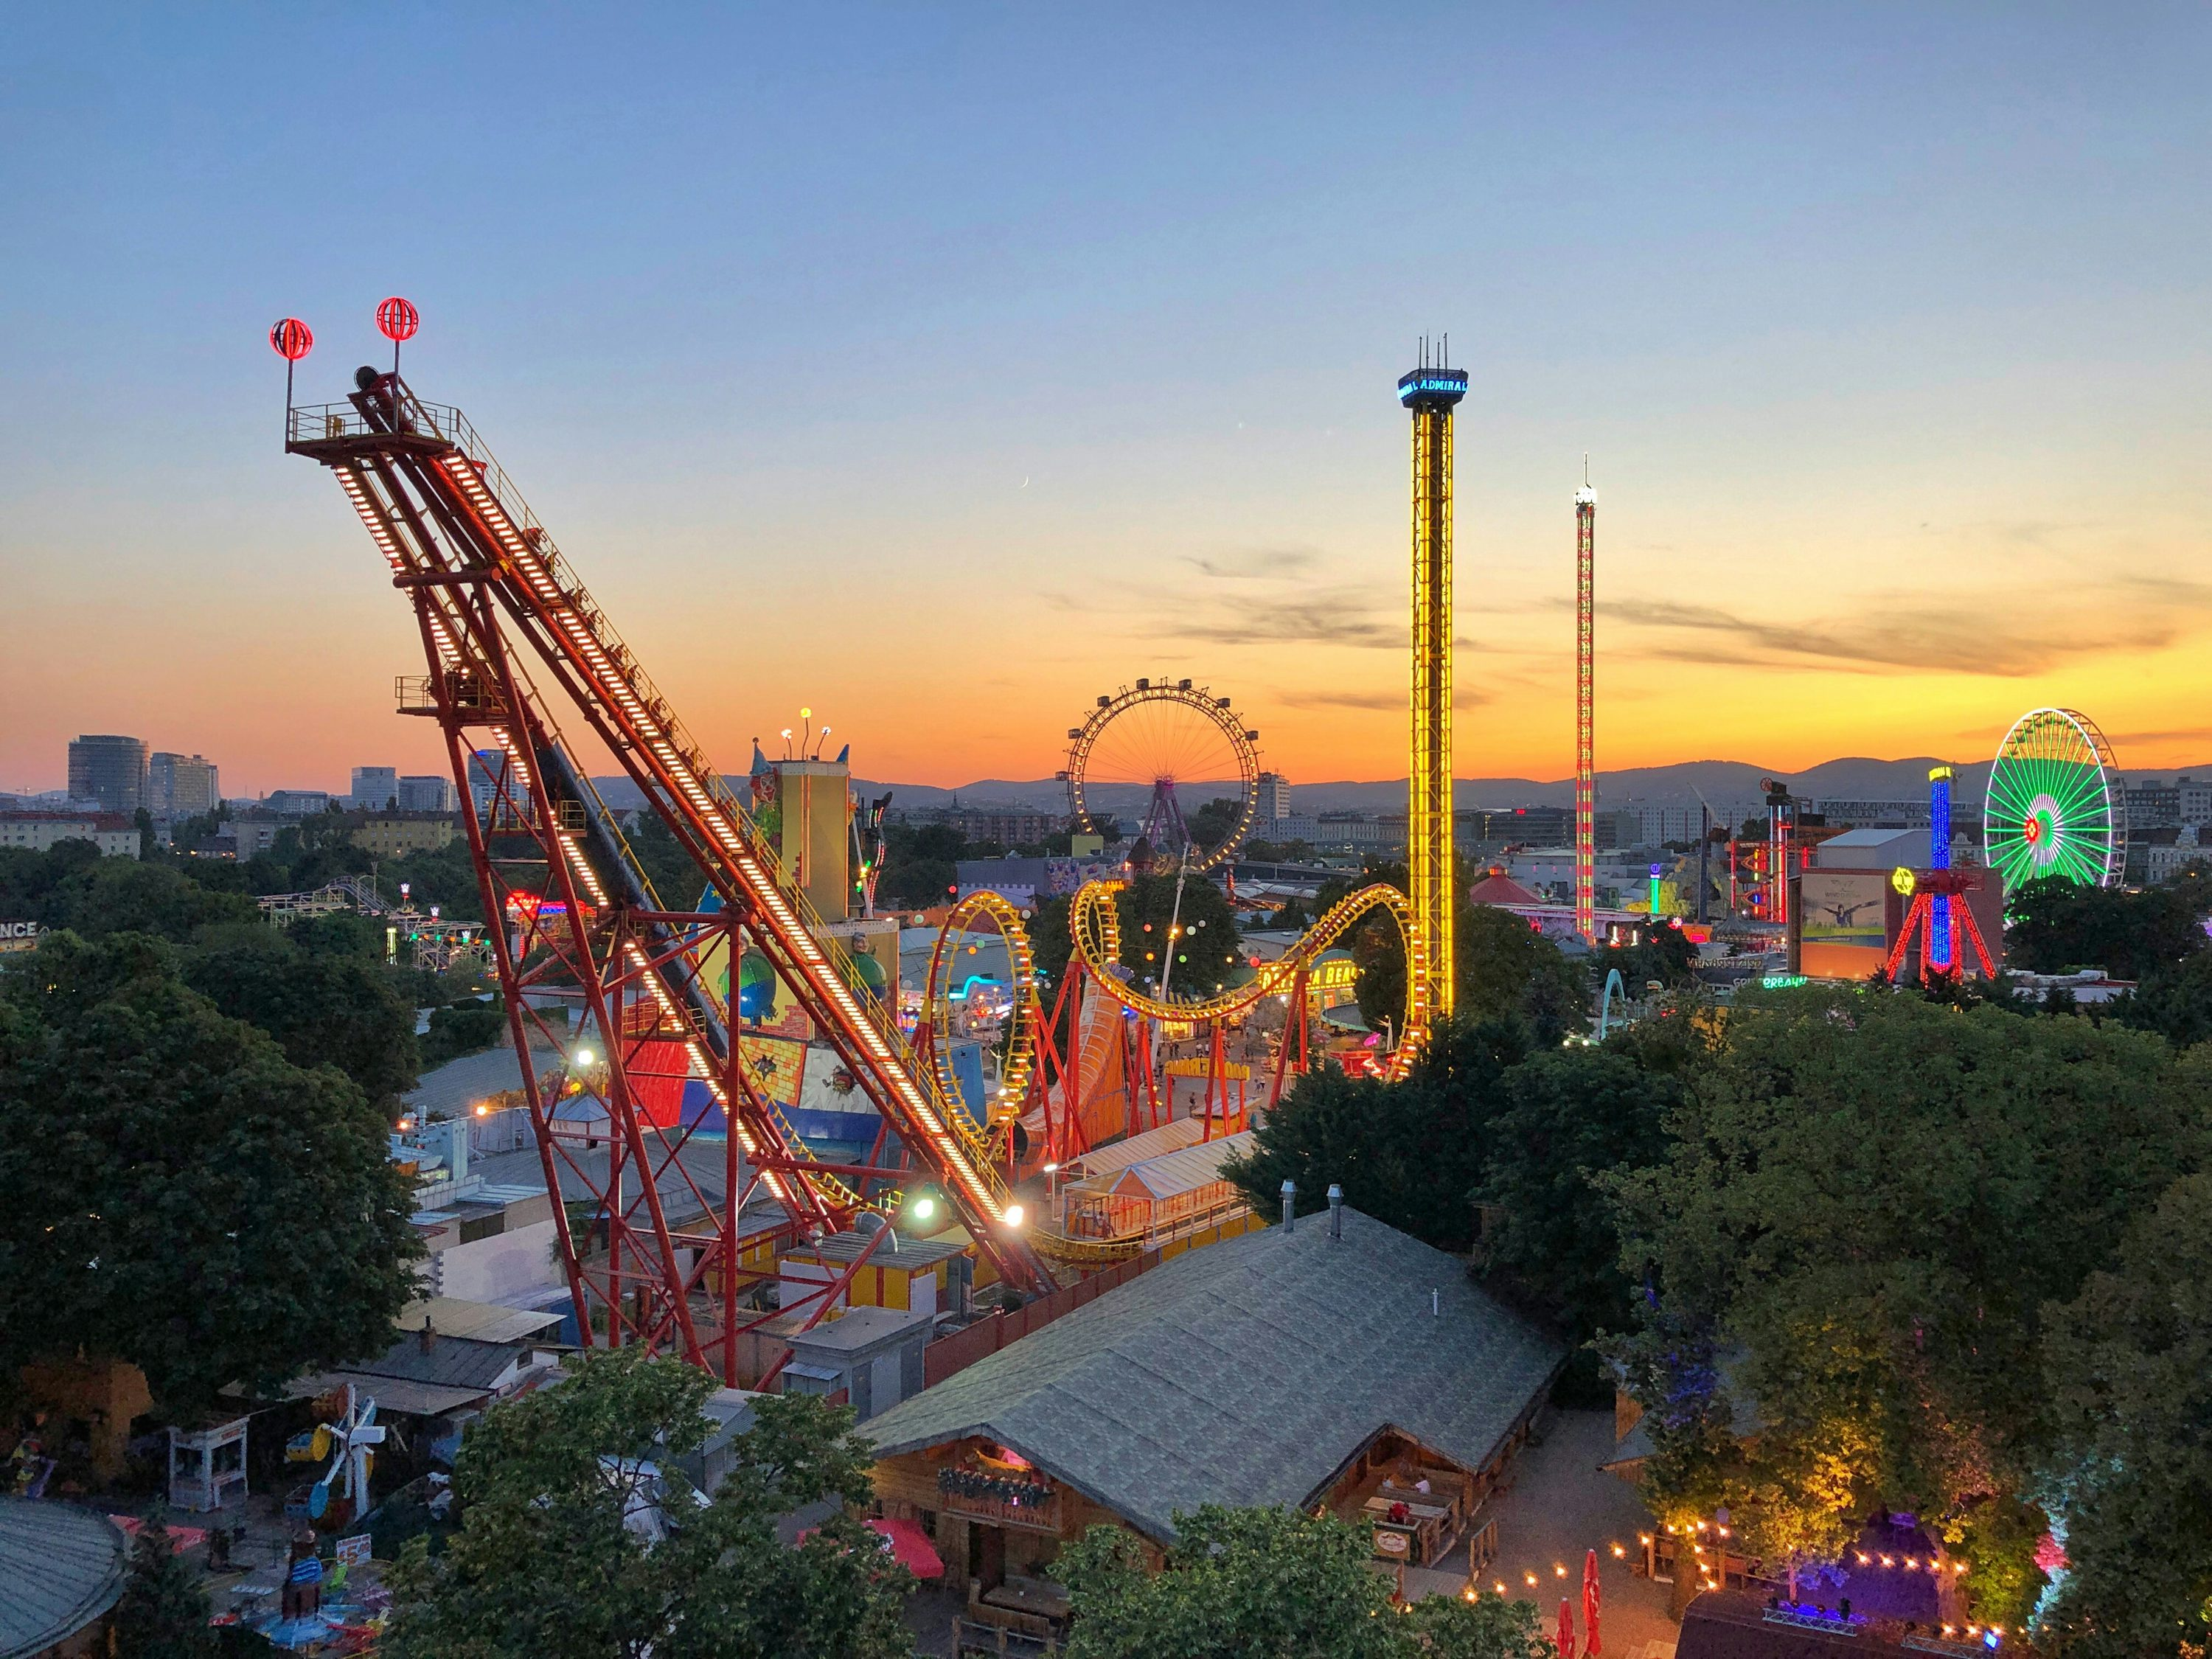
\includegraphics[width=1\textwidth]{themepark.jpg} % Puedes cambiar o eliminar esta imagen si no se usa
}
\author{Rodrigo Calderón, Álvaro Aguilar, Jaime Carrera}
\date{ 04/04/2025}

\begin{document}
\maketitle
\thispagestyle{empty}
\newpage
\tableofcontents
\newpage




\section{BUSINESS ORIENTATION}
The development of a theme park simulator not only holds academic or technical value, but also offers direct application within the business and operational environment of such facilities. This project is aimed at providing a decision-support tool for leisure managers, industrial engineers, operations supervisors, and experience designers in the tourism sector.
\subsection{Project Justification and Context}
Theme parks face numerous operational challenges: managing visitor flow, optimizing limited resources (ticket booths, turnstiles, staff, attractions), maximizing customer satisfaction, and adapting to fluctuations in demand. Implementing real-world solutions to evaluate decisions is costly, risky, and time-consuming.
This tool enables a realistic simulation of a full week of park operations, accounting for thousands of individual interactions between visitors, facilities, and timeframes. It allows experimenting with different configurations at no real cost—adjusting entry prices, extending or reducing opening hours, adding turnstiles, or modifying the range of available attractions. Additionally, it provides a controlled environment to analyze how these changes affect user behavior and the overall performance of the park.
\subsection{Simulator Impact and Usefulness}
The simulator has been designed to meet the following core objectives defined by the development team:
Reduce average waiting time by identifying operational bottlenecks.
Identify the most frequently used attractions and analyze saturation patterns.
Optimize the distribution of available resources (infrastructure, access points, staff).
Maximize visitor satisfaction by tracking the full experience.
Analyze the effects of specific decisions regarding flow, capacity, and ticketing.
A key functionality is its ability to detect improvement opportunities within the target audience.
\subsection{Practical Application in Real Environments}
This simulator can be applied to any type of amusement park, whether permanent or temporary. Its modular and configurable design allows it to adapt to large, medium, or small parks, regardless of their location or organizational structure. Typical implementation scenarios include:
Permanent theme parks with multiple zones and thematic areas.
\begin{itemize}
\item  Mobile or seasonal parks with variable operations.
\item  Family-oriented urban parks looking to expand their offer for children.
\item  Mixed leisure spaces with technological and digital attractions.
Thanks to its flexible architecture, the simulator can be customized based on:
\item  User profiles (age, ticket type, waiting time tolerance).
\item  Types of attractions and their specific configurations.
\item  Adaptable schedules, special promotions, and events.
\end{itemize}

\subsection{Future Projection of the Simulator as a Product}
This software is conceived as an evolving platform. In future versions, the following enhancements are planned:

\begin{itemize}
\item  Integration of machine learning modules for flow prediction.
\item  Real-time data visualization through interactive dashboards.
\item  Simulation of marketing strategies or campaigns during high-traffic periods.
\item  Expansion of behavioral logic based on psychological and social profiles.
\item  Development of a visual version with virtual visitor paths for presentations.
\end{itemize}

The ultimate goal is to consolidate the simulator as a professional-grade tool capable of improving, optimizing, and validating operational decisions in real amusement parks. A dynamic, adaptable, and data-driven system to transform both the visitor experience and operational efficiency.
\section{GENERAL SYSTEM DESCRIPTION}
The developed system is a discrete event simulator that represents the complete operation of a theme park over seven consecutive days. To achieve a realistic representation, the SimPy simulation environment was used, allowing the modeling of concurrent processes and shared resources—fundamental in environments with multiple points of interaction such as theme parks.
This simulator is aimed at both internal analysis and operational improvement of the park, enabling managers to evaluate visitor behavior under different configurations. One of its main objectives is to identify saturation points such as long queues at ticket booths or attractions, and to analyze the distribution of usage across the park’s various resources.
The simulation includes a fully dynamic configuration layer via a .csv file, which allows the following parameters to be defined: 

\begin{itemize}
\item  Number of ticket booths and entry turnstiles.
\item  Daily operating hours (opening and closing time).
\item  Total simulation duration per day.
\item  Ticket price.
\item  List of attractions, including capacity, duration, number of modules, and target audience.
\end{itemize}

Each day begins with the loading of this configuration, the initialization of the simulation environment, and the random generation of visitors. These visitors have specific characteristics (type, satisfaction level, fatigue, ticket type), and their behavior evolves throughout the day based on their experiences within the park.
Modular Structure of the System
The simulator has been designed following a modular and object-oriented approach, composed of the following main components:

\begin{itemize}
\item  ThemePark: Manages the complete flow of visitors, from arrival to departure, recording all intermediate events.
\item  TicketOffice: Manage entry resources (ticket booths and turntiles) and handle ticket purchase/validation processes, considering waiting times and potential dropouts.
\item  Attraction: Models the behavior of each individual attraction, including capacity, duration, queueing, wait-time penalties, and maintenance cycles.
\item  DataCollector: Logs all events occurring during the simulation, including visitor data, journey logs, usage times, wait times, ticket type, and exports the information to CSV files for analysis.
\item  Helper functions: Support functions for dynamic visitor generation, time formatting, and daily summary printing.
\end{itemize}

Daily Simulation Focus and Analytical Objectives
The park is simulated day by day, replicating realistic operational conditions. The environment enables:

\begin{itemize}
\item  Detection of the most popular attractions and assessment of their operational performance.
\item  Measurement of average time spent and usage by visitor profile.
\item  Evaluation of queue-reduction strategies through resource adjustment.
\item  Study of the impact of expanding the park’s offer for children and its effect on family attendance.
\end{itemize}

Each visitor may enter using an online ticket or through physical ticket booths. During their visit, they choose which attractions to visit, how long to stay, and when to leave the park, based on their fatigue and satisfaction levels. Every step of their journey is recorded for later analysis.
This system offers a solid foundation for future expansions and customizations, enabling its transformation into a high-level simulation tool applicable to a variety of real-world scenarios.

\section{USE CASES AND FUNCTIONALITIES}
The simulator has been designed with a realistic and practical approach to cover the main behavioral flows that occur in a real theme park. By modeling the various actors (visitors, attractions, ticketing) and shared resources, a system has been built that allows for observation, analysis, and data-driven decision-making.
\subsection{Main Use Cases}
The following use cases have been implemented in this first version of the simulator:
Visitor arrival simulation: Random generation with variable arrival rates depending on the time slot (peak hours during the first two hours, and decline at the end of the day).
Ticket purchase and validation: Management of entry flow through physical ticket booths and online ticket turnstiles. Waiting penalties and early exits if satisfaction drops too low.
Autonomous park navigation: Visitors randomly select valid attractions based on their profile, energy level, and satisfaction.
Interaction with attractions: Access control using SimPy resources (modules and staff), queuing, service usage, and penalties for delays. Includes maintenance cycles after certain usage thresholds.
Comprehensive event logging: Every visitor action is recorded (entry time, visited attraction, wait time, satisfaction, exit), enabling complete traceability.
Data analysis and export: At the end of each day, data is saved to .csv files for further analysis using tools like Excel or Pandas.
\subsection{Specific Features of the Simulator}

\begin{itemize}
\item  Capacity control in attractions based on modules and per-module limits.
\item  Queue management for ticket booths, turnstiles, and attractions, with realistic timing and stochastic variability.
\item  Early exit simulation when visitors experience excessive wait times or low satisfaction.
\item  Daily revenue calculation based on ticket booth sales.
\item  Impact measurement by visitor profile (children, teens, adults) to analyze attraction usage trends.
\item  Planning of critical events such as attraction maintenance, triggered under defined conditions (based on usage count).
\subsection{Strategic Applications of the Simulator}
The simulator acts as a diagnostic tool applicable to various operational needs in a theme park:
\item  Validate new pricing policies or entry configurations (discounts, extra ticket booths).
\item  Assess the potential of adding more child-focused attractions to attract family audiences.
\item  Optimize human resource allocation, especially in high-demand attractions.
\item  Forecast the impact of special promotions or events on park operations.
This event-driven simulation approach allows not only precise modeling of internal processes but also testing of different configurations to enhance the visitor experience and operational profitability.
\end{itemize}

\section{ARCHITECTURE AND TECHNICAL DESIGN}
The simulator's architecture is based on a modular, object-oriented model that enables the representation of different actors and processes involved in the operation of a theme park. Each module has a clearly defined responsibility and is designed to work in harmony with the SimPy simulation environment, which facilitates parallel process execution through discrete events.
The main components of the architecture, their relationships, and functional logic are detailed below.
\subsection{ThemePark Class}

\begin{itemize}
\item  Acts as the core class responsible for managing the complete visitor flow.
\item  Coordinates park entry through the TicketOffice.
\item  Controls individual visitor behavior throughout the day.
\item  Assesses each visitor’s fatigue and satisfaction to determine when they leave.
\item  Interacts with available attractions and logs events in the DataCollector.
\end{itemize}

Simplified pseudocode:


\begin{figure}[H]
    \centering
    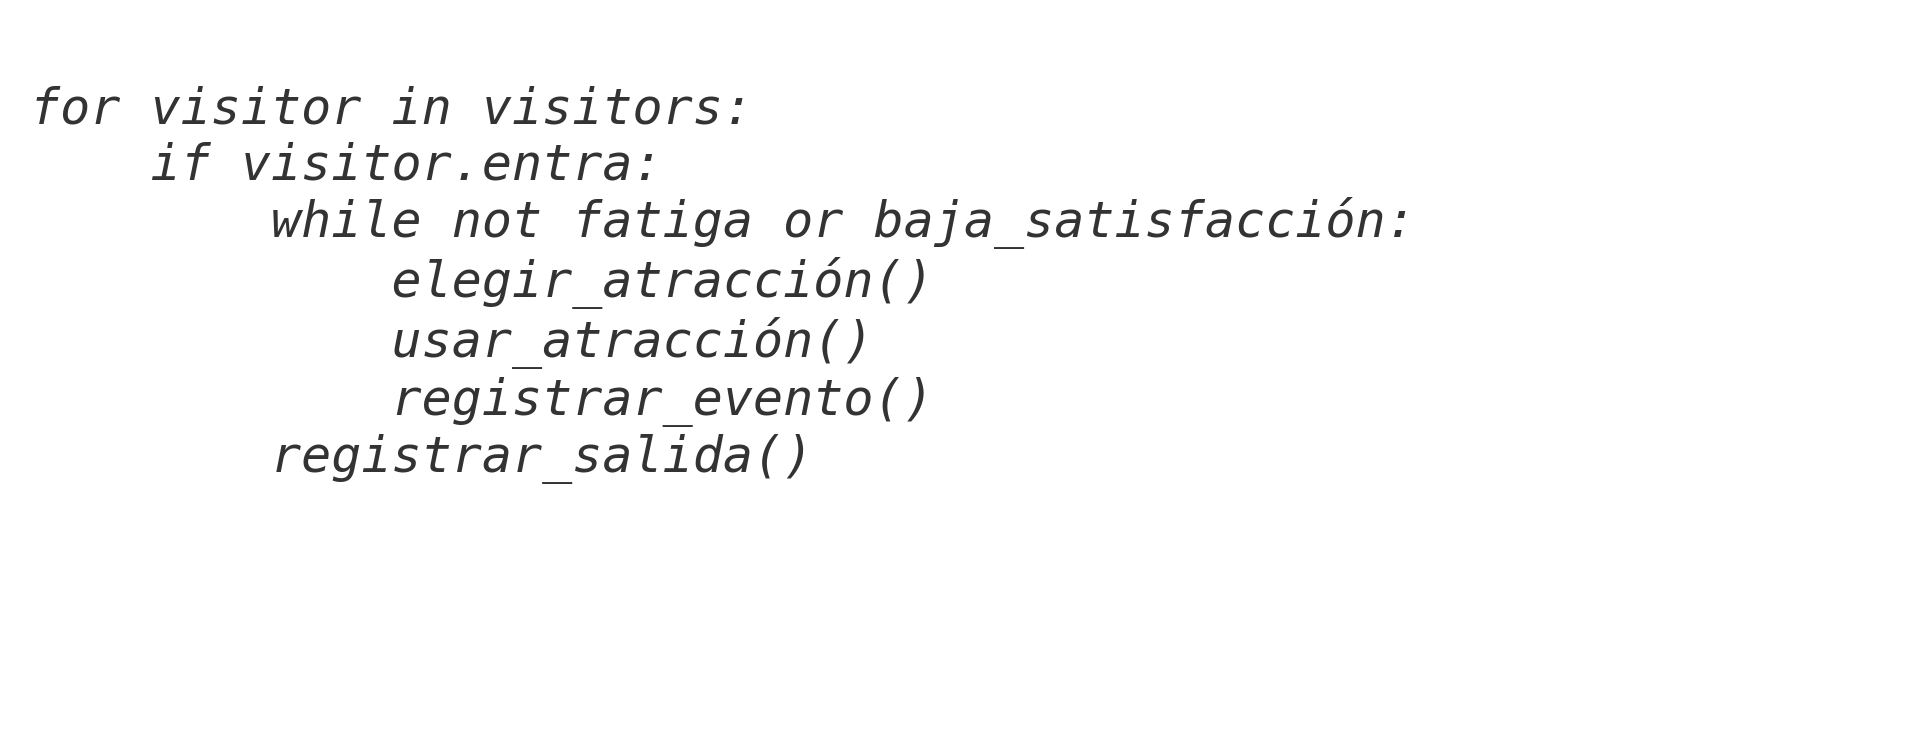
\includegraphics[width=0.75\textwidth]{visitor_pseudocode.png}
    \caption{Simplified pseudocode of visitor behavior during the simulation.}
    \label{fig:visitor-pseudocode}
\end{figure}

 \subsection{TicketOffice Class}

\begin{itemize}
\item Manages two SimPy resources: ticket booths (for purchasing tickets) and turnstiles (for entry validation).
\item Implements queue logic and satisfaction penalties for excessive waiting times.
\item Controls access based on ticket type (online or on-site).
\item Records successful sales, dropouts, and calculates daily revenue.
\item Key aspects:
\begin{itemize}
    \item Adaptive logic to prevent entry of visitors with low satisfaction levels.
    \item Stochastic waiting times ranging between 0.5 and 2 minutes.
    \item Ability to configure the number of ticket booths and turnstiles via the CSV file.
\end{itemize}
\end{itemize}

\subsection{DataCollector Class}

\begin{itemize}
\item Stores two main data structures:
\begin{itemize}
    \item \texttt{visitor\_data}: summary of each visitor (note: deprecated in current version).
    \item \texttt{journey\_log}: detailed log of all events during the simulation.
\end{itemize}
\item Exports the journey log to a CSV file for further analysis.
\item Records the following:
\begin{itemize}
    \item Successful and failed entries.
    \item Waiting and usage times.
    \item Attendance by ticket type.
\end{itemize}
\end{itemize}

% Imagen del visitante como figura externa
\begin{figure}[H]
    \centering
    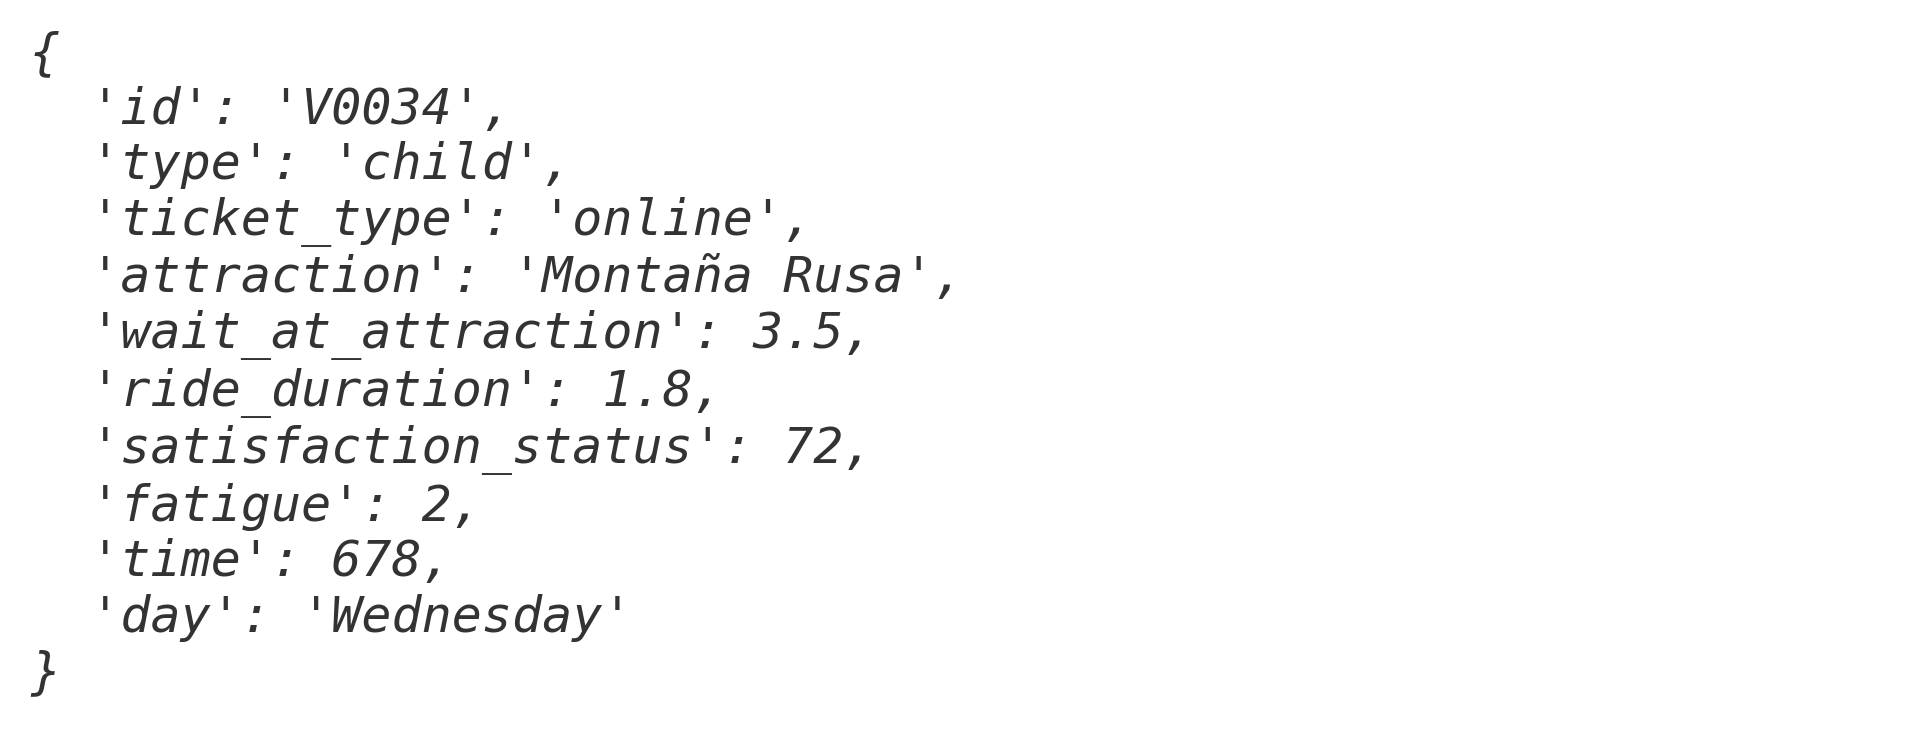
\includegraphics[width=0.65\textwidth]{visitor_data_dict.png}
    \caption{Example of a visitor event record in the simulation log.}
    \label{fig:visitor-data-dict}
\end{figure}

\subsection{Attraction Class}

\begin{itemize}
\item Controls access per module, duration per ride, and maintenance cycles.
\item Logs wait times, usage duration, popularity, and performance statistics.
\item Implements maintenance logic when a visitor usage threshold is reached.
\item Included logic:
\begin{itemize}
    \item Satisfaction penalty if the wait time exceeds 5 minutes.
    \item Random maintenance triggered after 400 to 600 uses.
    \item Staff and module resources allocated per attraction.
\end{itemize}
\end{itemize}

\subsection{Helper Functions (utils.helpers)}

\begin{itemize}
\item \texttt{generate\_visitors}: generates visitors stochastically based on profile and time of day.
\item \texttt{format\_time}: converts minutes to HH:MM format (useful for logs and visualization).
\item \texttt{print\_summary}: generates end-of-day reports including sales, timing, and attendance.
\end{itemize}

\textbf{Module Relationships:}

\begin{verbatim}
generate_visitors --> ThemePark --> TicketOffice
                                    |
                                    --> Attraction (usage)
                                    --> DataCollector (log)
\end{verbatim}

This architecture provides a solid foundation for future expansions, allowing the introduction of new visitor types, behavioral rules, economic models, or visual layers. Its modular design ensures maintainability and adaptability of the system in response to any operational change.

\section{WORK METHODOLOGY (AGILE)}

The development of the simulator was carried out using an iterative and incremental work approach, based on the principles of Agile methodology. It was structured into a series of weekly sprints, with functional deliveries at the end of each cycle and a constant system of review and continuous improvement.

\subsection{Work Phases}
(The detailed table of phases can be added here if needed.)

\subsection{Tools Used}
\begin{itemize}
\item Version control: GitHub, to ensure traceability of changes.
\item Planning: Trello and Gantt charts for task assignment and scheduling.
\item Development environment: Visual Studio Code and Jupyter Notebooks.
\item Peer review: Code reviews were conducted at the end of each sprint.
\end{itemize}

\subsection{Meetings and Team Dynamics}
\begin{itemize}
\item Sprint planning meetings at the beginning of each week.
\item Progress review meetings every 3 days.
\item Weekly retrospectives to improve work processes.
\item Continuous communication via shared repositories and collaboration spaces.
\end{itemize}

\subsection{Adaptability and Iterative Improvements}

During the development process, improvements were identified and incorporated iteratively:

\begin{itemize}
\item Implementation of maintenance logic after identifying recurring congestion.
\item Enhancement of visitor generation based on time-of-day adaptation.
\item Removal of the \texttt{visitor\_data.csv} file to simplify the system.
\end{itemize}

This approach enabled the creation of a functional product from the early stages, rapid adaptation to changes, improved code quality, and a clear vision of the final objective: to build a flexible, professional tool for decision-making in amusement park management.





\section{TEAM ROLES}
This project was developed through the coordinated participation of a multidisciplinary team, where each member assumed clear responsibilities in different phases of the process. The role structure allowed for effective time management, prioritization of deliverables, and assurance of product quality.

\begin{figure}[H]
    \centering
    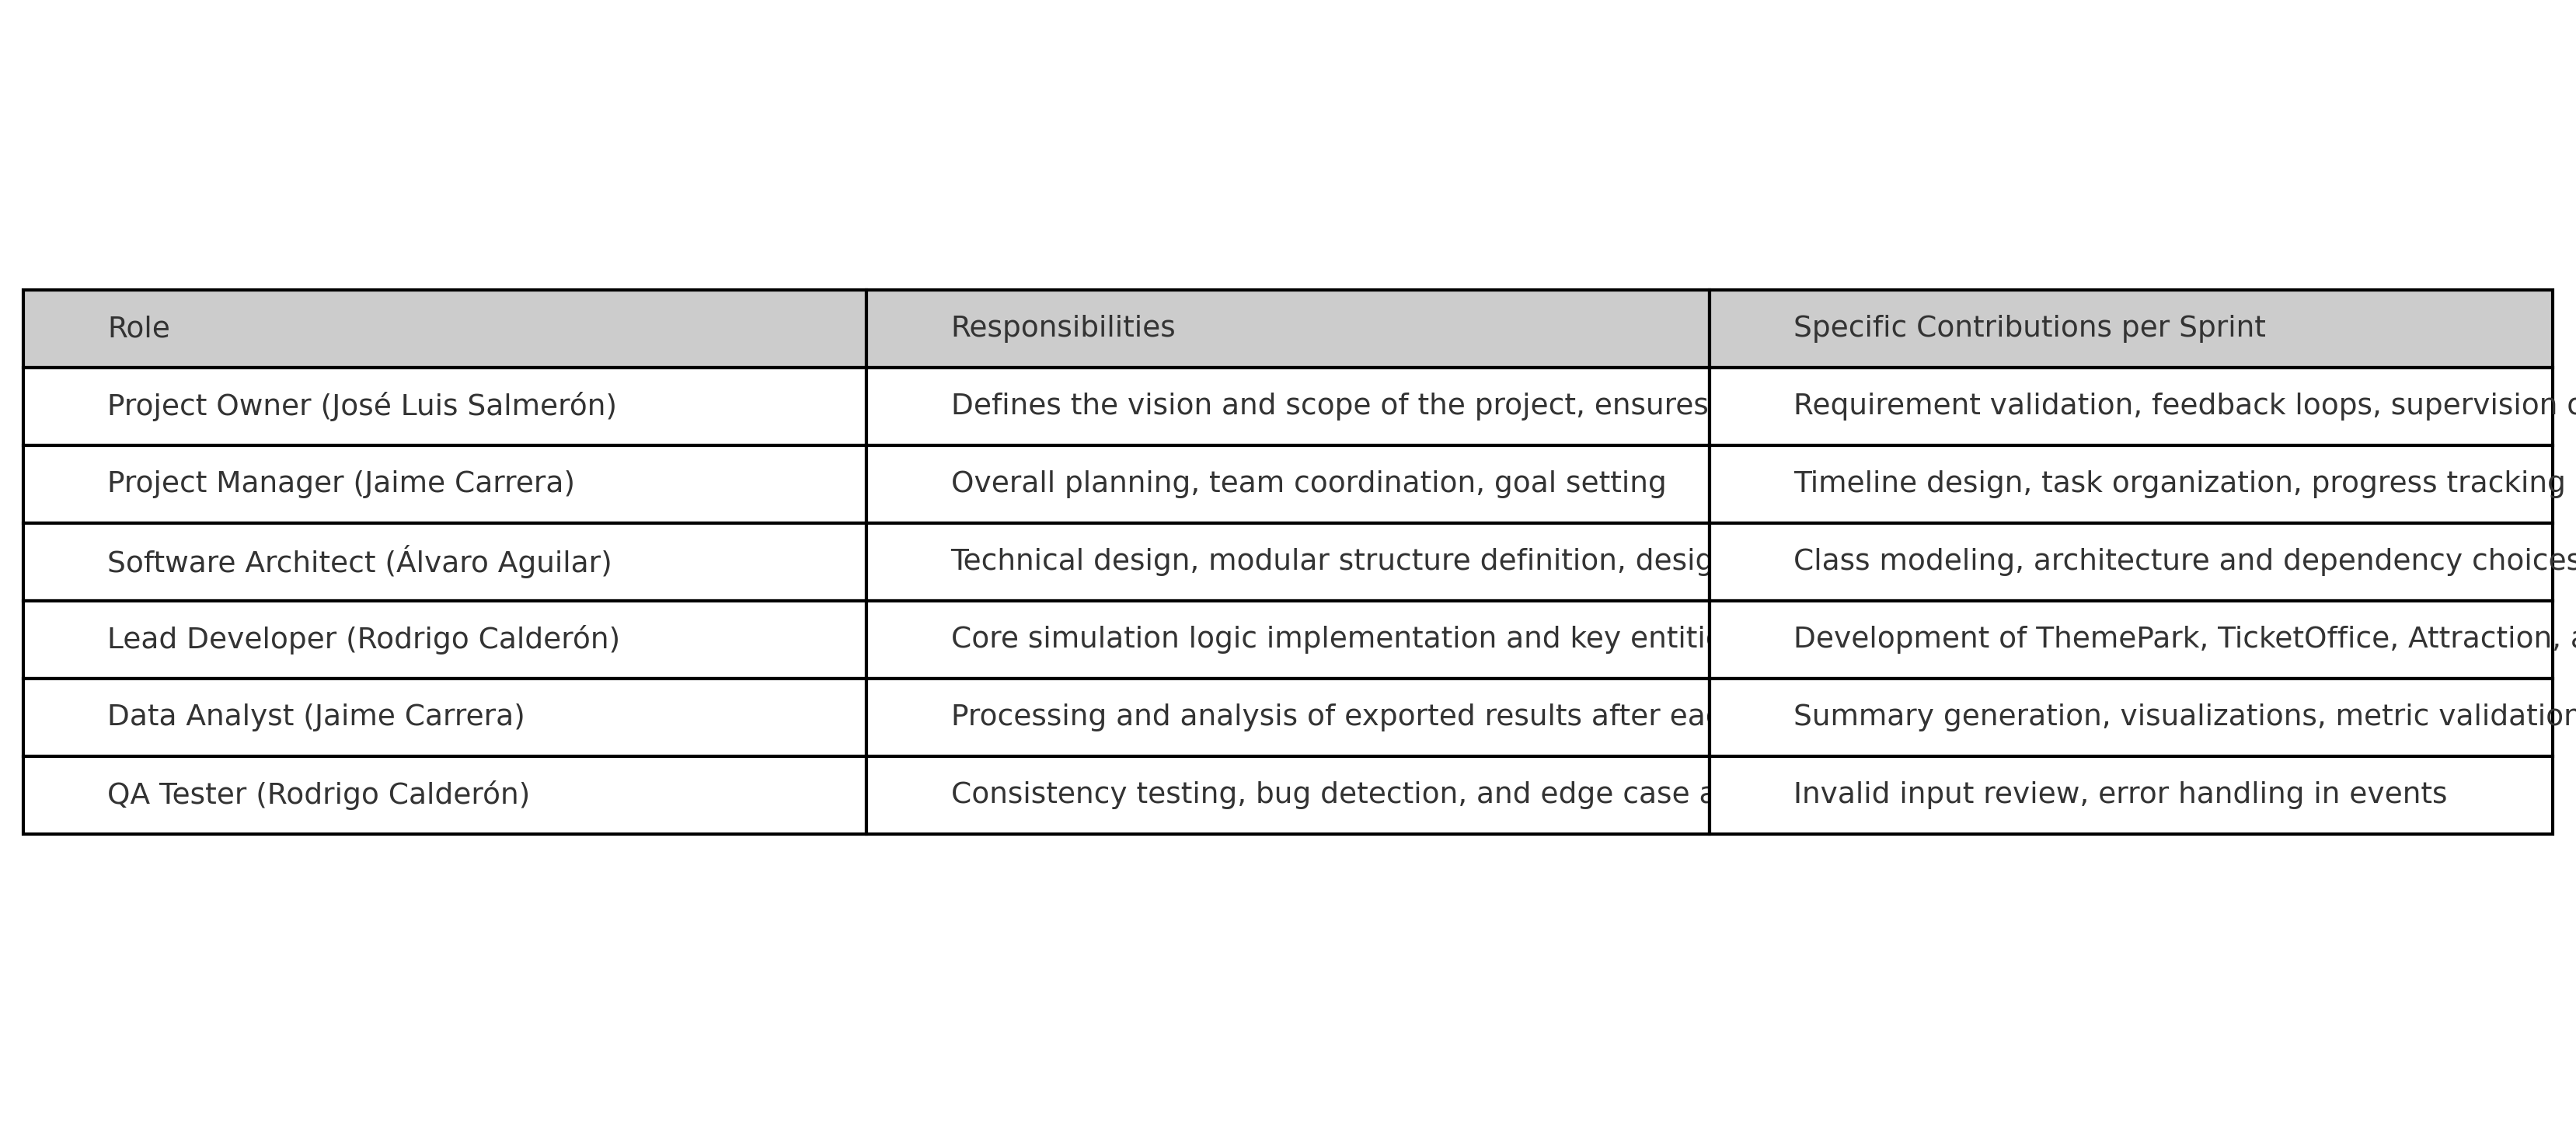
\includegraphics[width=\textwidth]{team_roles_english.png}
    \caption{Team roles and specific contributions during development sprints.}
    \label{fig:team-roles}
\end{figure}


\section{TECHNICAL COMPLEXITY AND DESIGN CONSIDERATIONS}

Implementing the simulator involved several technical challenges, requiring in-depth analysis of software design, process modeling, event control, and data handling. This section outlines the key aspects that define the complexity of the project and the design decisions made to ensure its robustness and scalability.

\subsection{Technology Selection}

SimPy was chosen as the simulation engine due to its ability to model discrete event processes in a simple yet powerful way. Unlike more visual but rigid libraries, SimPy allows for customized logic, queue handling, wait times, limited resources, and concurrency.

Additional tools and technologies used:
\begin{itemize}
    \item Python: Main language for its versatility, readability, and large ecosystem.
    \item CSV: Lightweight format to parameterize the park and export simulation results.
\end{itemize}

\subsection{Input Validation and System Robustness}

All core classes include validations for data type and structure. Examples include:
\begin{itemize}
    \item Verifying non-empty lists when instantiating attractions.
    \item Ensuring numeric and positive values for capacities, prices, or durations.
    \item Capturing and handling exceptions when using SimPy resources.
\end{itemize}

\subsection{Concurrency and Shared Resource Handling}

Using \texttt{simpy.Resource} enabled accurate simulation of simultaneous access to:
\begin{itemize}
    \item Ticket booths
    \item Entry turnstiles
    \item Attraction modules
    \item Attraction staff (operators)
\end{itemize}

These resources generate queues and wait times based on real demand. The design considers:
\begin{itemize}
    \item Limited and configurable capacity from the CSV.
    \item Satisfaction penalties for long waits.
    \item Retries, early exits, and blocked access when applicable.
\end{itemize}

\subsection{Dynamic Penalties and Adaptive Behavior}

Visitor satisfaction is affected by environmental variables:
\begin{itemize}
    \item Waiting times over 5 minutes reduce satisfaction based on duration.
    \item Fatigue increases after each attraction, influencing park stay.
    \item Visitors with low satisfaction may leave before completing their journey.
\end{itemize}

This logic creates emergent, unpredictable behaviors that enrich the simulation experience.

\subsection{Maintenance Control and Attraction States}

Attractions alternate between “operational” and “maintenance” states. This process is triggered when a configurable visitor threshold is reached. During maintenance:
\begin{itemize}
    \item The attraction is temporarily disabled.
    \item A random repair time is simulated.
    \item After completion, maintenance counters are reset.
\end{itemize}
\subsection{Export, Persistence, and Post-Simulation Analysis}

Currently, the system exports the \texttt{visitor\_journey.csv} file, which records all events in detail. This file can be analyzed using tools such as Pandas, Power BI, or Excel.

Example of exported CSV content:

\begin{figure}[H]
    \centering
    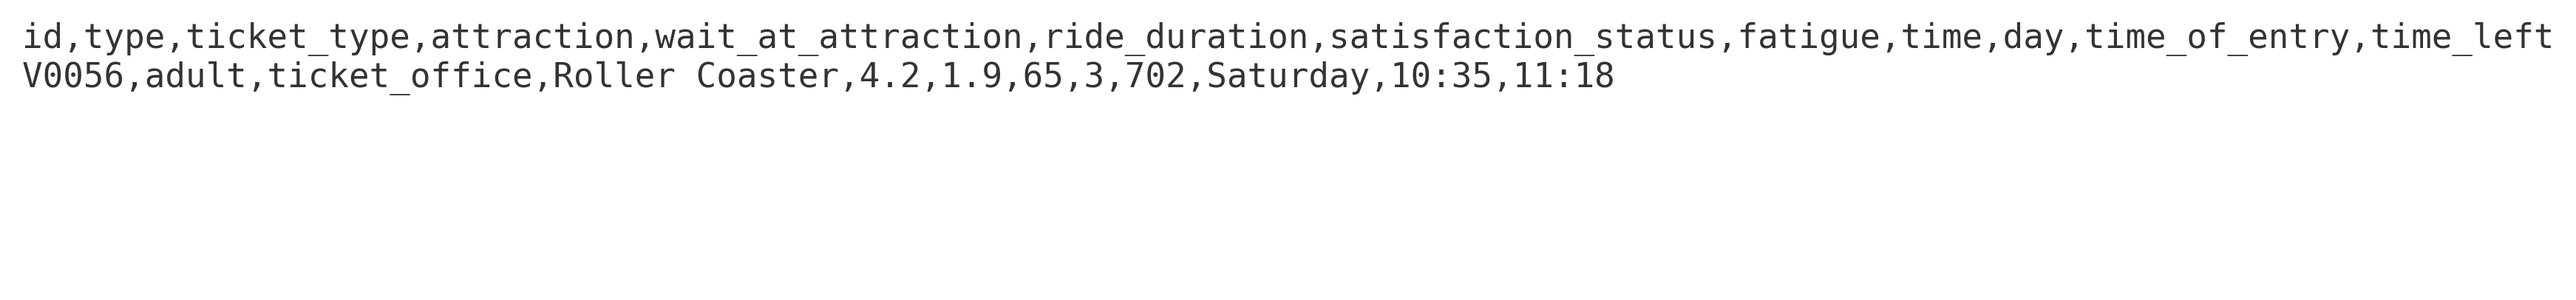
\includegraphics[width=1\textwidth]{visitor_csv_record.png}
    \caption{Example of exported visitor data in CSV format.}
    \label{fig:visitor-csv-record}
\end{figure}


\subsection{Future Considerations}

\begin{itemize}
    \item Use of relational databases to manage simulation histories.
    \item Real-time dashboards for integrated visualization.
    \item Modularization into packages to facilitate maintenance and reusability.
    \item Multi-scenario support to compare configurations and evaluate improvements.
\end{itemize}

\section{CONFIGURATION AND RESULTS ANALYSIS}

This section presents a detailed analysis of the data collected during the weekly simulation of the theme park. The objective is to identify key behavioral patterns among visitors, evaluate the effectiveness of operational configurations, and provide data-driven recommendations for improving the overall park experience.

A variety of statistical and visualization techniques were used, including correlation analysis, distributional plots, segmentation by visitor attributes, and clustering.

\subsection{Correlation Analysis}

\begin{figure}[H]
    \centering
    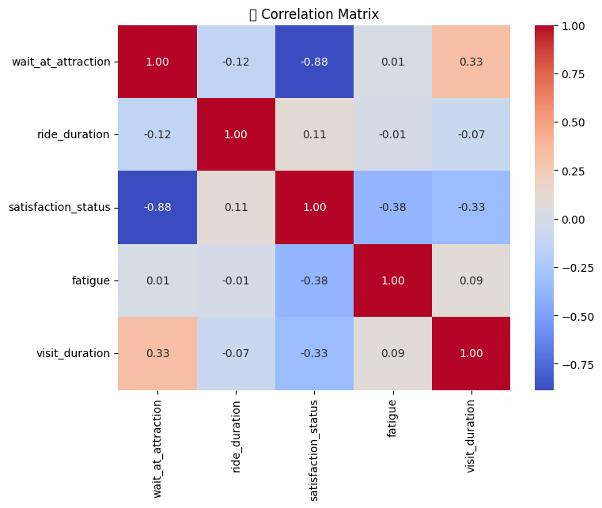
\includegraphics[width=1\textwidth]{correlation_matrix.png}
    \caption{Correlation Matrix}
    \label{fig:correlation-matrix}
\end{figure}

The following correlation matrix summarizes the relationships between key visitor experience variables, such as wait time, satisfaction, fatigue, visit duration, and ride duration.

\begin{itemize}
    \item \textbf{Wait Time and Satisfaction (r = -0.88):} A strong negative correlation indicates that longer wait times significantly reduce visitor satisfaction. Reducing queues should be a priority.
    \item \textbf{Wait Time and Visit Duration (r = 0.33):} Visitors who remain longer in the park tend to experience higher wait times. This could be due to visiting during peak hours or engaging in a larger number of attractions.
    \item \textbf{Satisfaction and Fatigue (r = -0.38):} Higher fatigue levels are associated with lower satisfaction, reinforcing the importance of visitor comfort.
    \item \textbf{Satisfaction and Visit Duration (r = -0.33):} Longer visits tend to correlate slightly with reduced satisfaction, likely due to cumulative fatigue or reduced novelty.
    \item \textbf{Ride Duration Correlations:} Ride duration has weak or negligible correlations with other metrics, indicating that it is not a strong predictor of satisfaction or fatigue.
    \item \textbf{Fatigue and Other Variables:} Fatigue shows weak correlation with most variables, except for satisfaction. This suggests that fatigue is more complex and influenced by individual pacing or experience.
\end{itemize}

\subsection{Distribution of Visitor Metrics}

The following histograms illustrate the distribution of key metrics to better understand general visitor behavior and experience throughout the week.

\begin{figure}[H]
    \centering
    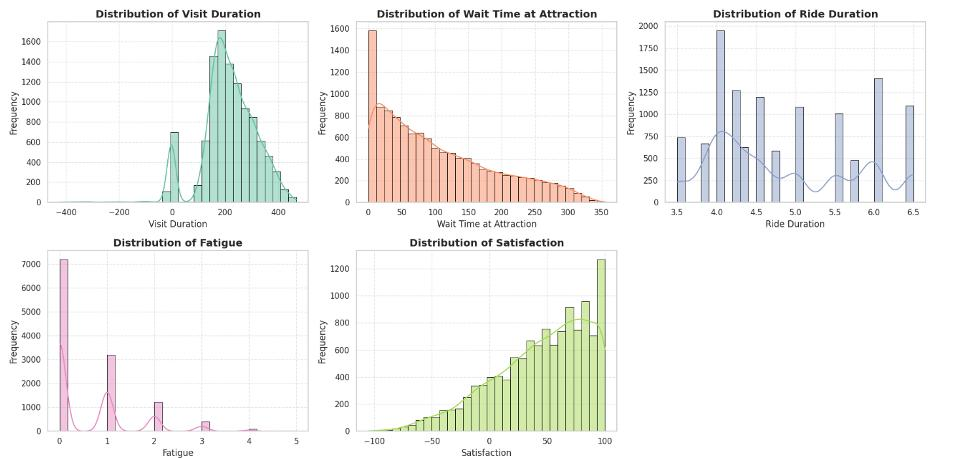
\includegraphics[width=1\textwidth]{distribution_plots.png}
    \caption{Distribution of Visitor Metrics}
    \label{fig:distribution-metrics}
\end{figure}

\begin{itemize}
    \item \textbf{Visit Duration:} The distribution is right-skewed, with the majority of visitors spending between 100 and 300 minutes in the park. Outliers with extremely short or negative values suggest data quality issues.
    \item \textbf{Wait Time at Attractions:} Most visitors experience relatively low wait times. However, the long right tail indicates that some visitors experience significantly longer queues, particularly during peak hours.
    \item \textbf{Ride Duration:} A multimodal distribution reflects predefined ride durations. Peaks indicate standardized categories (e.g., 4–6 minutes), consistent with fixed attraction schedules.
    \item \textbf{Fatigue:} Most visitors report low levels of fatigue, with minimal dispersion. A few higher values may correspond to more intensive usage patterns.
    \item \textbf{Satisfaction:} Satisfaction scores are concentrated above 70, with some negative outliers pointing to possible recording or processing errors.
\end{itemize}

\subsection{Comparison by Visitor Type (Adults vs. Children)}

This section compares experience metrics between adult and child visitors, focusing on duration of stay, satisfaction levels, and fatigue.

\begin{figure}[H]
    \centering
    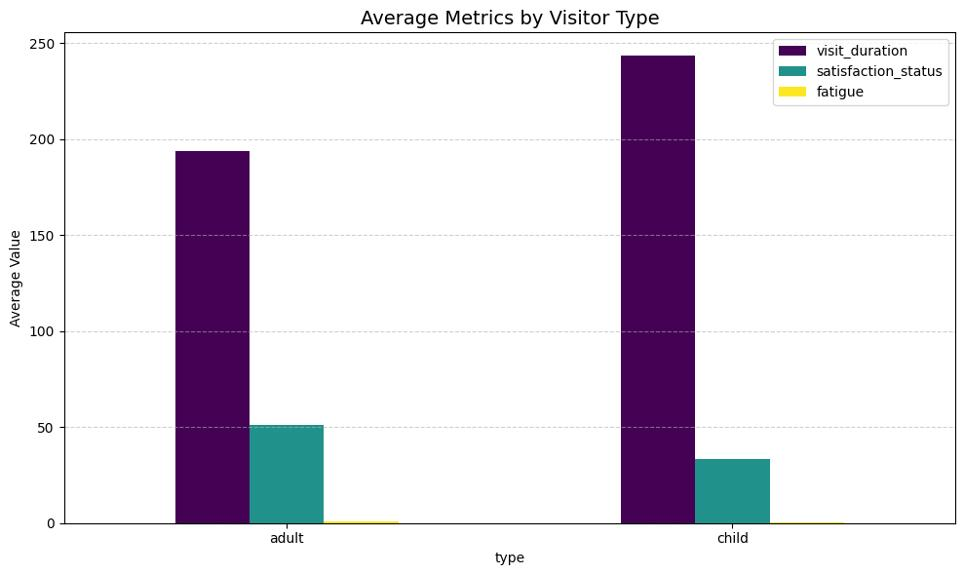
\includegraphics[width=1\textwidth]{average_visitor_type.png}
    \caption{Average metrics by visitor type}
    \label{fig:average_visitor_type}
\end{figure}

\begin{itemize}
    \item \textbf{Visit Duration:} Children tend to stay longer than adults. This may be due to broader engagement with child-specific attractions or family visits.
    \item \textbf{Satisfaction:} Adults report significantly higher satisfaction. This may indicate that existing services are better aligned with adult expectations, or that children are more affected by discomfort or waiting.
    \item \textbf{Fatigue:} Both groups report low fatigue levels, with children showing slightly less fatigue, possibly due to different pacing.
    \item \textbf{Conclusion:} The experience is currently more favourable for adults. Improvements in child-specific engagement and comfort may help balance satisfaction across demographics.
\end{itemize}

\subsection{Impact of Ticket Type}
This analysis compares the impact of ticket acquisition method (online vs. ticket office) on visit duration and satisfaction.

\begin{figure}[H]
    \centering
    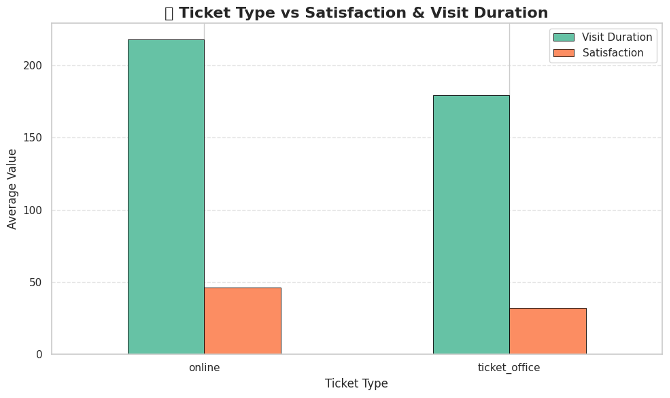
\includegraphics[width=1\textwidth]{ticket_type_comparison.png}
    \caption{Comparison of ticket type with average visit duration and satisfaction level.}
    \label{fig:ticket-type-comparison}
\end{figure}

Visit Duration:
Online ticket holders tend to remain in the park longer, possibly due to streamlined entry and better planning.
Satisfaction:
Visitors who purchased tickets online report higher satisfaction, likely due to reduced entry friction and greater convenience.
Conclusion:
The data highlights a clear benefit in promoting online ticketing:
It correlates with longer engagement in the park.
It is associated with higher visitor satisfaction.
Improving the digital experience and incentivizing online sales could further enhance operational flow and visitor sentiment.
\subsection{Visitor Clustering (K-Means Analysis)}
A behavioral segmentation was conducted using K-Means clustering based on standardized metrics such as visit duration, wait time, satisfaction, and fatigue.

\begin{figure}[H]
    \centering
    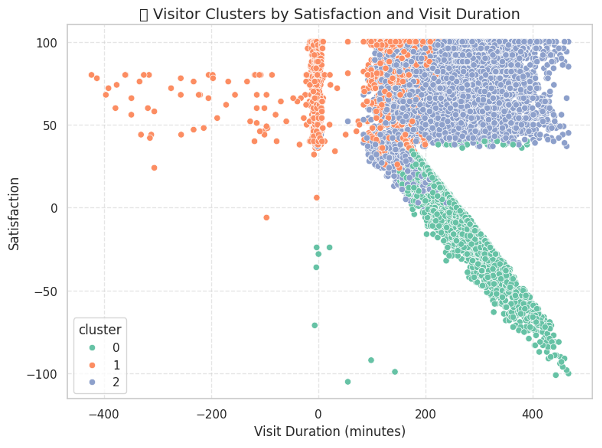
\includegraphics[width=1\textwidth]{visitor_clusters.png}
    \caption{Segmentation of visitors using clustering based on visit duration and satisfaction level.}
    \label{fig:visitor-clusters}
\end{figure}

Cluster Descriptions:
Cluster 0 (Short Visit, High Satisfaction):
Visitors in this group have short visits but report high satisfaction. They likely focus on a few targeted experiences.
Cluster 1 (Long Visit, Low Satisfaction):
This group stays the longest but reports low or even negative satisfaction. Factors may include long queues or exhaustion. This group represents a risk for negative feedback.
Cluster 2 (Balanced Experience):
Visitors show moderate-to-long durations with consistently high satisfaction. This cluster represents the target behavior pattern for optimal park flow.
Observations:
Data anomalies (e.g., negative values) were present and require correction.
Longer stays do not necessarily correlate with higher satisfaction.
Segmentation allows for differentiated strategies: improve Cluster 1, maintain Cluster 2, and optimize efficiency for Cluster 0.


\subsection{Boxplot Analysis by Age Group}
Boxplots were used to compare visit duration, satisfaction, and fatigue between adults and children.

\begin{figure}[H]
    \centering
    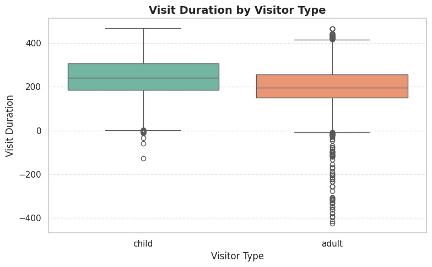
\includegraphics[width=1\textwidth]{visit_duration_by_type.png}
    \caption{Visit duration by visitor type (children vs. adults).}
    \label{fig:visit-duration-type}
\end{figure}

Visit Duration:
Children stay longer on average, with a wider interquartile range. Outliers, including negative durations, should be addressed through data cleaning.

\begin{figure}[H]
    \centering
    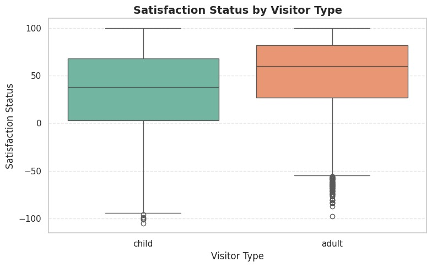
\includegraphics[width=1\textwidth]{satisfaction_by_type.png}
    \caption{Satisfaction level by visitor type (children vs. adults).}
    \label{fig:satisfaction-type}
\end{figure}

Satisfaction:
Adults consistently show higher satisfaction. Children’s results are more dispersed, indicating a greater sensitivity to negative factors.


\begin{figure}[H]
    \centering
    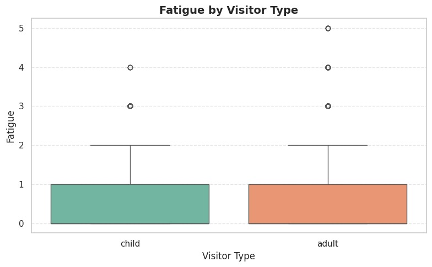
\includegraphics[width=1\textwidth]{fatigue_by_type.png}
    \caption{Fatigue levels by visitor type (children vs. adults).}
    \label{fig:fatigue-type}
\end{figure}

Fatigue:
Both groups exhibit low levels of fatigue, suggesting balanced pacing. Isolated high outliers may be linked to individual behavior.
Conclusion:
The experience is more optimized for adult visitors. Additional efforts should be made to enhance the child experience, reduce dissatisfaction, and maintain low fatigue levels.

\subsection{Weekly Wait Time Patterns}
A violin plot was used to visualize how attraction wait times fluctuate by day of the week.

\begin{figure}[H]
    \centering
    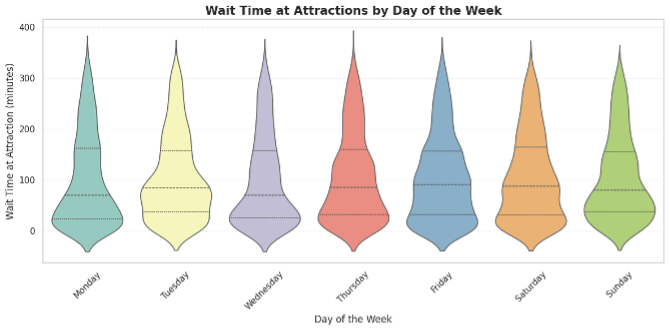
\includegraphics[width=1\textwidth]{wait_time_by_day.png}
    \caption{Wait time at attractions by day of the week.}
    \label{fig:wait-time-by-day}
\end{figure}

Weekends (Saturday–Sunday):
Highest variability and longest wait times due to peak visitor volume.
Tuesday:
Lowest and most consistent wait times, making it the optimal day for a balanced park experience.
Monday and Wednesday:
Moderate wait times and stable distributions, suggesting efficient management.
Thursday and Friday:
An upward trend in wait times, signalling the beginning of weekend congestion.
Conclusion:
Visitor load follows a predictable weekly cycle. Operational planning should prioritize weekend crowd management while leveraging midweek periods—particularly Tuesday—for smoother and higher-quality visitor experiences.
\end{document}